    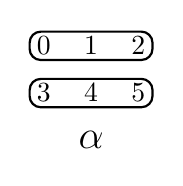
\begin{tikzpicture}[scale=.6]          
                % B_0
          \foreach \j in {0,1,2} {
            \draw (\j -1, 0.5) node {$\j$};
            \pgfmathtruncatemacro{\x}{\j+3}
            \draw (\j -1, -0.5) node {$\x$};
          }
 \draw[font=\Large] (0,-1.5) node {$\alpha$};
      \draw[rounded corners,thick,\ifdot] (-1.3,-.8) rectangle (1.3,-.2);
      \draw[rounded corners,thick,\ifdot] (-1.3,.8) rectangle (1.3,.2);
    \end{tikzpicture}
    \hfill
    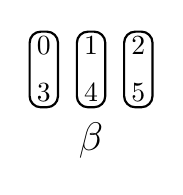
\begin{tikzpicture}[scale=.6] 
                % B_0
          \foreach \j in {0,1,2} {
            \draw (\j -1, 0.5) node {$\j$};
            \pgfmathtruncatemacro{\x}{\j+3}
            \draw (\j -1, -0.5) node {$\x$};
          }
 \draw[font=\Large] (0,-1.5) node {$\beta$};
      \draw[rounded corners,thick,\ifdot] (-1.3,-.8) rectangle (-.7,.8);
      \draw[rounded corners,thick,\ifdot] (-.3,-.8) rectangle (.3,.8);
      \draw[rounded corners,thick,\ifdot] (1.3,-.8) rectangle (.7,.8);
    \end{tikzpicture}
    \hfill
    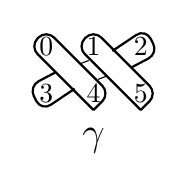
\begin{tikzpicture}[scale=.6] 
                % B_0
          \foreach \j in {0,1,2} {
            \draw (\j -1, 0.5) node {$\j$};
            \pgfmathtruncatemacro{\x}{\j+3}
            \draw (\j -1, -0.5) node {$\x$};
          }
 \draw[font=\Large] (0,-1.5) node {$\gamma$};
      \draw[rounded corners,thick,\ifdot] (1,-.85) to (1.35,-.5) to  (-0,.85) to (-.35,.5) to (1,-.85);
      \draw[rounded corners,thick,\ifdot] (0,-.85) to (0.35,-.5) to  (-1,.85) to (-1.35,.5) to (0,-.85);
      \draw[rounded corners,thick,\ifdot] (.8,.05) to (1.37,.35) to  (1.1,.87) to (.4,.4);
      \draw[rounded corners,thick,\ifdot] (-.8,-.05) to (-1.37,-.35) to  (-1.1,-.87) to (-.4,-.4);
      \draw[\ifdot] (-0.1,.2) to (-.28,.13);
      \draw[\ifdot] (0.1,-.2) to (.28,-.13);
    \end{tikzpicture}
    \hfill
    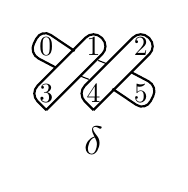
\begin{tikzpicture}[scale=.6]
                % B_0
          \foreach \j in {0,1,2} {
            \draw (\j -1, 0.5) node {$\j$};
            \pgfmathtruncatemacro{\x}{\j+3}
            \draw (\j -1, -0.5) node {$\x$};
          }
 \draw[font=\Large] (0,-1.5) node {$\delta$};
      \draw[rounded corners,thick,\ifdot] (-1,-.85) to (-1.35,-.5) to  (0,.85) to (.35,.5) to (-1,-.85);
      \draw[rounded corners,thick,\ifdot] (0,-.85) to (-0.35,-.5) to  (1,.85) to (1.35,.5) to (0,-.85);
      \draw[rounded corners,thick,\ifdot] (-.8,.05) to (-1.37,.35) to  (-1.1,.87) to (-.4,.4);
      \draw[rounded corners,thick,\ifdot] (.8,-.05) to (1.37,-.35) to  (1.1,-.87) to (.4,-.4);
      \draw[\ifdot] (0.1,.2) to (.28,.13);
      \draw[\ifdot] (-0.1,-.2) to (-.28,-.13);
    \end{tikzpicture}
